%********************************************
\chapter{Ejemplo de cosas que se pueden hacer}\label{ch:introducción}
%********************************************

\marginpar{Ejemplo comentario al margen}

Ejemplo cita 1 \citeauthor{bringhurst:2002} % no sale enlace

Ejemplo cita 2 \citep{bringhurst:2002} % si sale

Ejemplo cita 3 \cite{bringhurst:2002} % si sale

Enlace a pie de pagina \footnote{Pie de página}

\emph{Curiva}, \texttt{maquina}, \textit{itálica}, \spacedallcaps{All Caps},  \textsc{Small Caps}, \spacedlowsmallcaps{Low Small Caps}.

Comentarios de algo de \verb|tex|.

Ejemplo en latín \eg

Acrónimos: \ac{UML}, \acs{UML} ,\acf{UML}, \acp{UML}

\paragraph{Párafro:} Lorem ipsum dolor sit amet, consectetur adipiscing elit. Integer vitae dapibus orci. Cras vel nunc mattis, lobortis sapien sit amet, pharetra enim. Nullam bibendum libero in sodales faucibus. Nullam risus mi, vehicula in metus ut, tristique molestie mauris. Nullam a sem augue. Sed tincidunt rutrum leo at tempor.

\subsection{Subsección}
\graffito{Comentario justo al lado del título de la sección}

\begin{table}[h]
  \myfloatalign
  \begin{tabularx}{\textwidth}{Xl} \toprule
    \tableheadline{head1 expandido} & \tableheadline{head2}  \\
    \midrule
    1 & 2 \\
    3 & 4 \\
    %postulant quo & westeuropee & sanctificatec \\
    \midrule
    5 & 6 \citeauthor{knuth:1976} \\
    \bottomrule
  \end{tabularx}
  \caption[Ejemplo de tabla 1]{Ejemplo de tabla 1}  \label{tab:example}
\end{table}

\begin{tabular}{ll}
$\rho$       & rho \\
$ \delta x$  & delta x \\
Ejemplo de tabla 2 &
\end{tabular}

% enlarga esta página (por abajo 2 cent): \enlargethispage{2cm}

\begin{figure}[h]
  \myfloatalign
  \subfloat[Imagen 1]
  {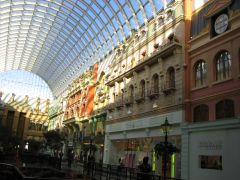
\includegraphics[width=.45\linewidth]{gfx/example_1}} \quad
  \subfloat[Imagen 2]
  {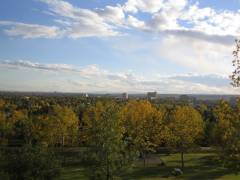
\includegraphics[width=.45\linewidth]{gfx/example_2}}
  \caption[Ejemplo figure]{Ejemplo figure}\label{fig:example}
\end{figure}

\begin{equation}
  x = 2 \quad (\textrm{texto})
\end{equation}

\begin{eqnarray*}
  x = 3 \\
  y = 4
\end{eqnarray*}

Referencia: \autoref{tab:example} y \autoref{ch:introducción}

\clearpage % new page
